
\section{Contrôle de la caméra}
  \begin{frame}
   \frametitle{Contrôle de la caméra}


\begin{figure}[H]
  \centering
     \begin{itemize}
    \item Classe dédiée au traitement des requêtes HTTP envoyées à la caméra
    \begin{itemize}
      \item Codes réponses différents selon la commande
      \item Parsage réalisé pour certaines réponses
    \end{itemize}
    \item Chargement de la configuration et des fonctionnalités supportées
    \item Adaptation de l'interface aux modèles de caméra Axis
   	\end{itemize}
   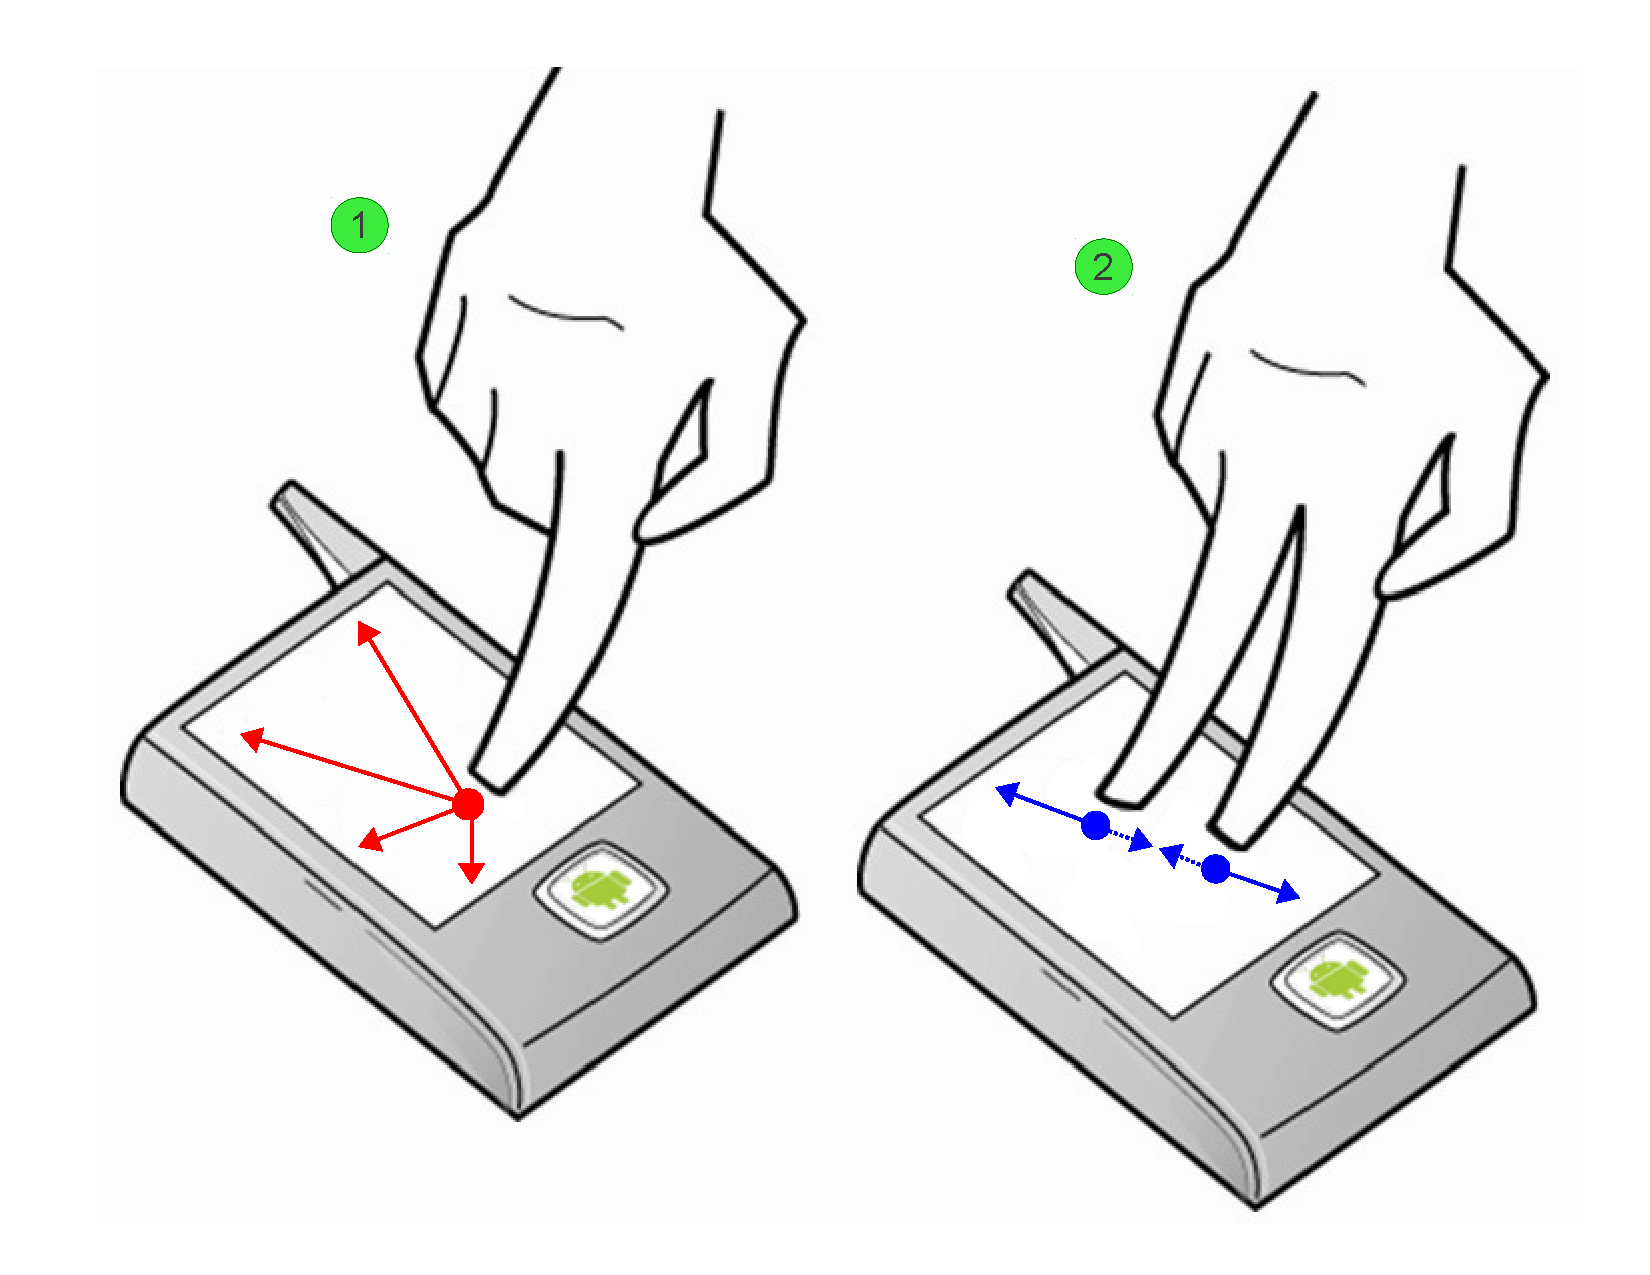
\includegraphics[scale=0.25]{Images/ImageSlide8.pdf}
  \end{figure}  

  \end{frame}
